\subsection{Cuantificador de Entropías Implementado en FPGA}
\label{ssecCuantiImpFPGA}

En esta Sección se describe la implementación de un sistema de medición de entropías.
El diseño fue optimizado para ser implementado en un microcontrolador simple y pequeño, conservando una precisión aceptable.
El sistema permite medir entropías a señales generadas internamente por código y a señales externas analógicas muestreadas.
Se utilizó la placa de desarrollo \textit{M1AFS-embedded kit} de ACTEL.
En la FPGA (\textit{Field Programmable Gate Array}) se instanció un microcontrolador 8051 al que se programó en lenguaje C.
Se detalla el diseño del \textit{hardware} y \textit{software} y los resultados obtenidos.
Al momento hay muy poca bibliograf\'ia sobre implementaciones en \textit{hardware} de estos cuantificadores \cite{DeMicco2013}.

La entropía es empleada en diversas aplicaciones, como por ejemplo, en la detección de anomalías en flujos de datos IP \cite{Gu2005,Wagner2006, actelM1AFS1500}.
En \cite{Subramanya2008} se presentó un diseño y simulación en FPGA de un cuantificador de entropía, sin embargo, actualmente no hay disponibles implementaciones en \textit{hardware} de este cuantificador.

En esta tesis se implementó un sistema que calcula la entropía para la PDF asociada a una serie de datos.
Se analizan PDFs causales y no causales.
Los datos pueden tener un origen digital (generados mediante códigos), o bien provenir del muestreo de señales analógicas.
Se utilizó la placa de desarrollo \textit{M1AFS-embedded kit}, basado en el chip \textit{M1AFS1500} que se destaca por tener un bloque analógico embebido en el mismo encapsulado de la FPGA.
Luego, se verificó la exactitud numérica del cuantificador implementado comparando sus resultados con un programa patrón.
A partir del máximo error detectado se determinó la exactitud numérica del sistema.

\subsubsection{\textit{Hardware} Implementado}
\label{sec:Hardware}

El diseño del \textit{hardware} se basó en el que provee ACTEL en \cite{Core8051sH}, basado en el microcontrolador 8051, interfaces y periféricos.
Fue realizado con el paquete de programas \textit{Libero~Soc~v11.3\textsuperscript\copyright} de ACTEL.
Se utilizó la placa de desarrollo \textit{M1AFS-EMBEDDED-KIT} que contiene una FPGA \textit{M1AFS1500} de ACTEL y periféricos \cite{actelM1AFS1500}.
El chip \textit{M1AFS1500} contiene embebido un bloque analógico que consiste en nueve adaptadores direccionables de cuatro entradas cada uno, un multiplexor analógico de 32 entradas y un conversor analógico-digital configurable.

El sistema implementado puede dividirse en tres etapas principales como se muestra en la Figura \ref{Fig:Sistema}: una primera etapa de Adquisición de datos, que convierte a palabras digitales las señales del mundo analógico, una Lógica de Cálculo, que se vale de la memoria SRAM para llevar a cabo los cálculos y coordinar las interfaces y una etapa de Presentación de resultados, que envía los resultados de la medición a una computadora a través de la interfaz \textit{USB-to-UART}.
%
\begin{figure}
	\centering
	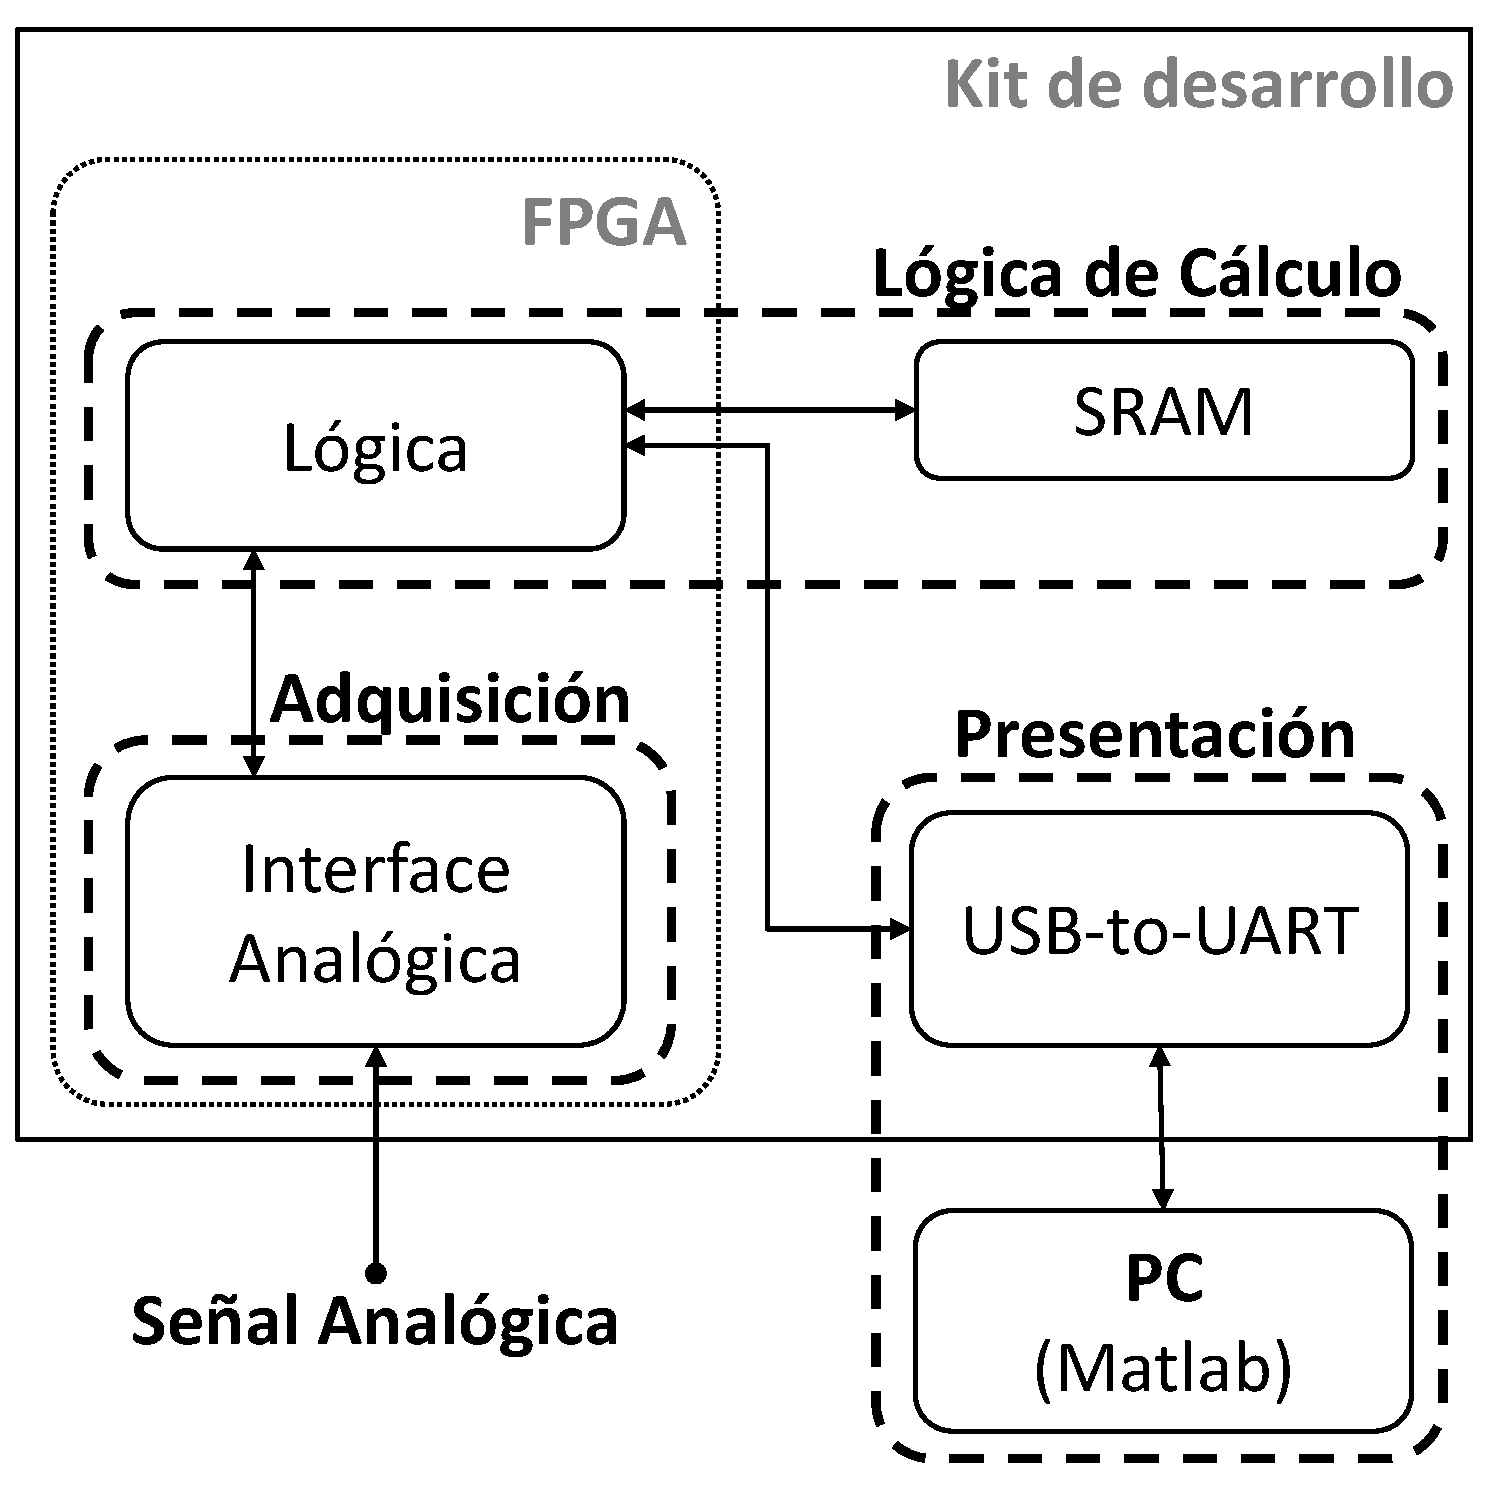
\includegraphics[width=.8\columnwidth]{Sistema.pdf}\\
	\caption{Esquema del sistema completo.}\label{Fig:Sistema}
\end{figure}

\begin{enumerate}
	\item \textit{Etapa de Adquisición:}
	
	Para ingresar los datos analógicos a ser evaluados utilizamos la entrada de tensión $AV2$ del \textit{Analog~Quad~2} del bloque analógico.
	Se encuentra direccionada en el canal siete del multiplexor analógico y fue configurada para un rango de tensiones de entrada de 0~V a 4~V.
	El conversor analógico-digital se configuró con una resolución de 12~bits.
	En este primer prototipo la frecuencia de muestreo máxima alcanzada fue de 16~ks/s limitada por el retardo necesario en el procesamiento de la lógica.
	
	\item \textit{Lógica de cálculo:}
	
	En esta etapa se realizan los cálculos y la sincronización entre periféricos.
	En la Figura \ref{fig:logica} pueden verse los bloques principales que la componen.
	%
	\begin{figure}
		\centering
		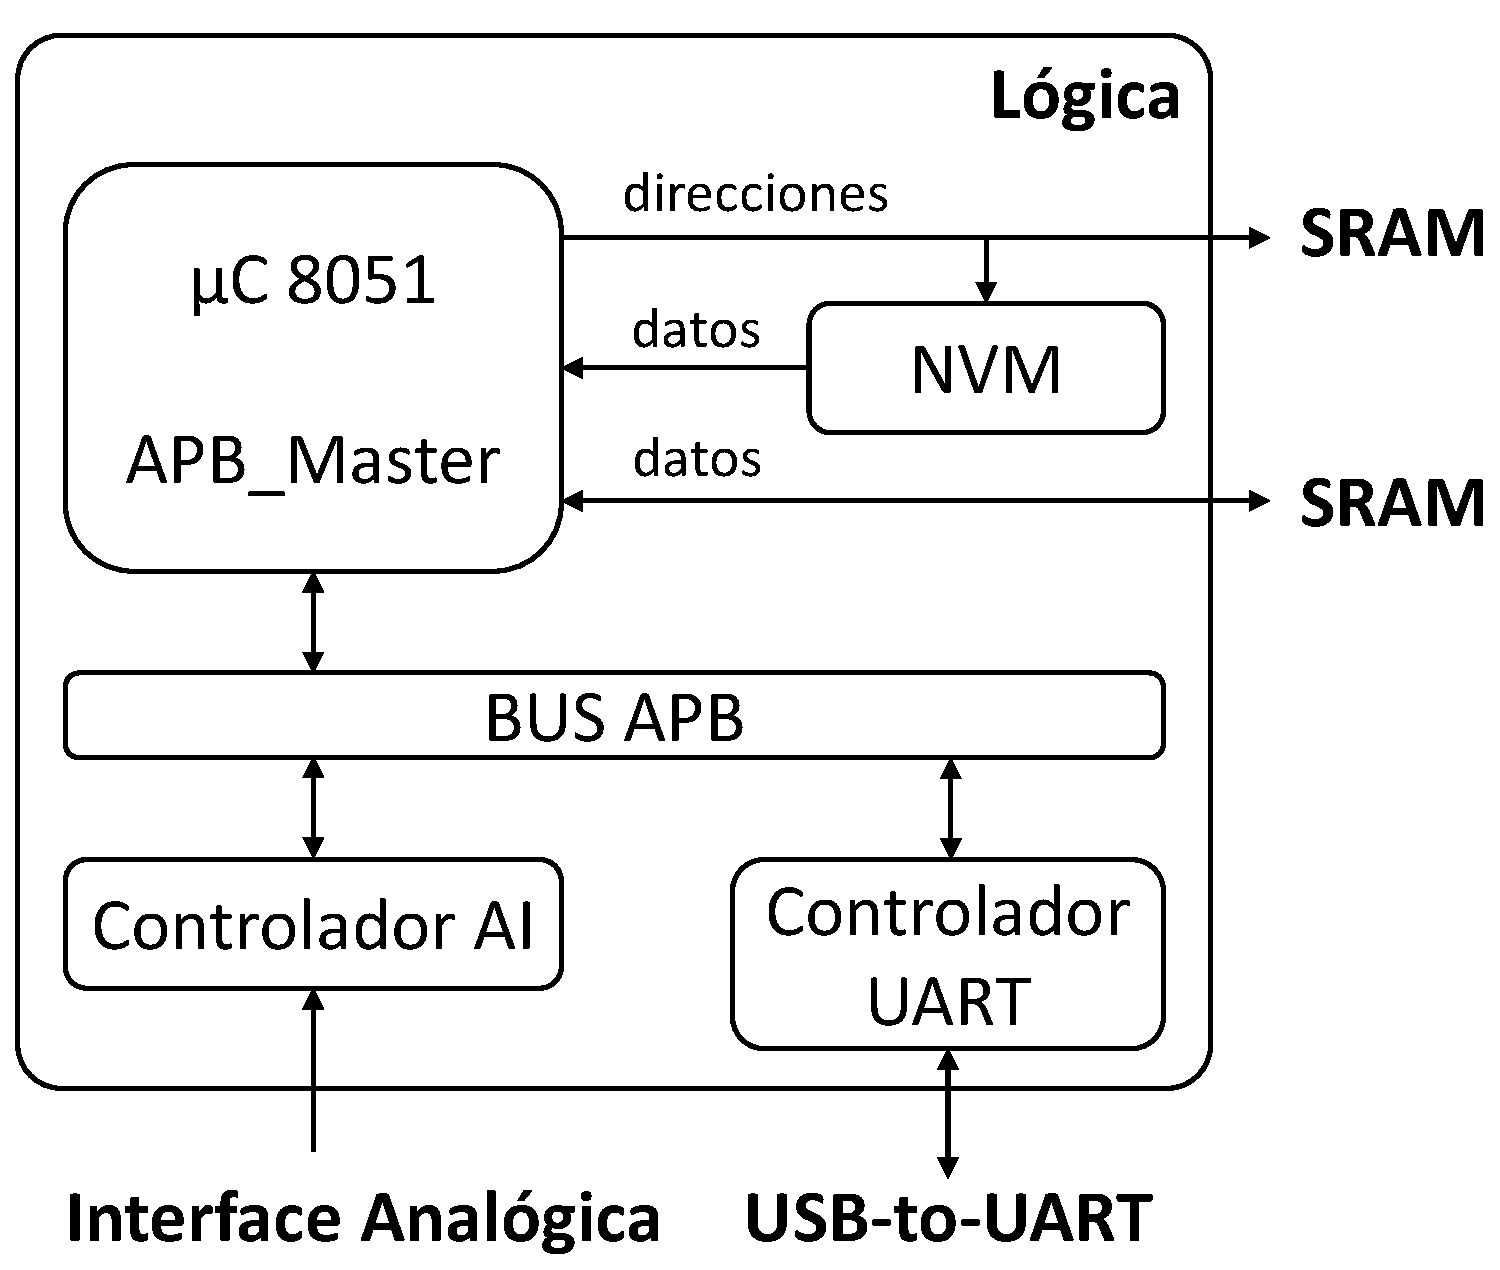
\includegraphics[width=.75\columnwidth]{Logica.pdf}\\
		\caption{Detalle de la lógica de cálculo.}\label{fig:logica}
	\end{figure}
	
	El núcleo de la implementación es un \textit{Core} 8051 que provee ACTEL en su catálogo de librerías.
	Se trata de un microcontrolador que contiene la lógica principal del microprocesador 8051 de Intel, sin sus periféricos.
	Este micro tiene una arquitectura Von Newman con un bus de direcciones de 16~bits, lo que limita nuestro diseño a $64~KB$ de memoria de código y $64~KB$ de memoria de datos.
	
	Sobre este microcontrolador corre el programa que realiza los cálculos presentados en la Sección \ref{sec:ITQs}.
	Se encarga de, a partir de los datos de entrada, obtener las PDFs ($BP$ e $hist$) y de realizar los cálculos para la obtención de las entropías, según la Ecuación \ref{shannon-disc-normalizada}.
	El \textit{software} implementado se describe más detalladamente en la Sección \ref{sec:Software}.
	
	La memoria de código es una memoria no volátil (NVM) implementada con los bloques flash internos de la FPGA.
	Ocupa las direcciones desde 0x0000 hasta 0xFFFF y se escribe con el contenido de un archivo en formato hexadecimal durante la compilación.
	
	Las funcionalidades del sistema son ampliadas mediante la conexión de periféricos a través de la interfaz APB.
	
	Para realizar la comunicación con la PC utilizamos el \textit{Controlador UART}.
	La salida de este bloque es dirigida hacia afuera de la FPGA y se conecta a un chip \textit{USB-to-UART} que se encuentra soldado a la placa del kit de desarrollo.
	
	El bloque analógico es controlado por el \textit{Controlador AI}, que direcciona y sincroniza sus entradas.
	
	\item \textit{Presentación:}
	
	La etapa de Presentación de los datos involucra al chip adaptador \textit{USB-to-UART} que se encuentra en la placa de desarrollo y es manejado tanto por el programa que corre en la FPGA como por el \textit{software} que corre sobre la PC.
	El chip adaptador \textit{USB-to-UART} es el responsable de adaptar la entrada-salida UART de la lógica a una entrada-salida USB estándar mediante la cual es posible interactuar con la PC.
	Por otra parte el programa que corre en la PC se encarga de la interfaz con el usuario y es descripto en detalle en la siguiente Sección.
	
\end{enumerate}

\subsubsection{\textit{Software} Implementado}
\label{sec:Software}

El funcionamiento del sistema se logra mediante la interacción de dos programas.
Uno corriendo en la PC y otro en el microcontrolador implementado en la FPGA.
Puede verse un diagrama de flujo de ambos programas y la interacción entre ellos en la Figura
\begin{figure}[htpb]
	\centering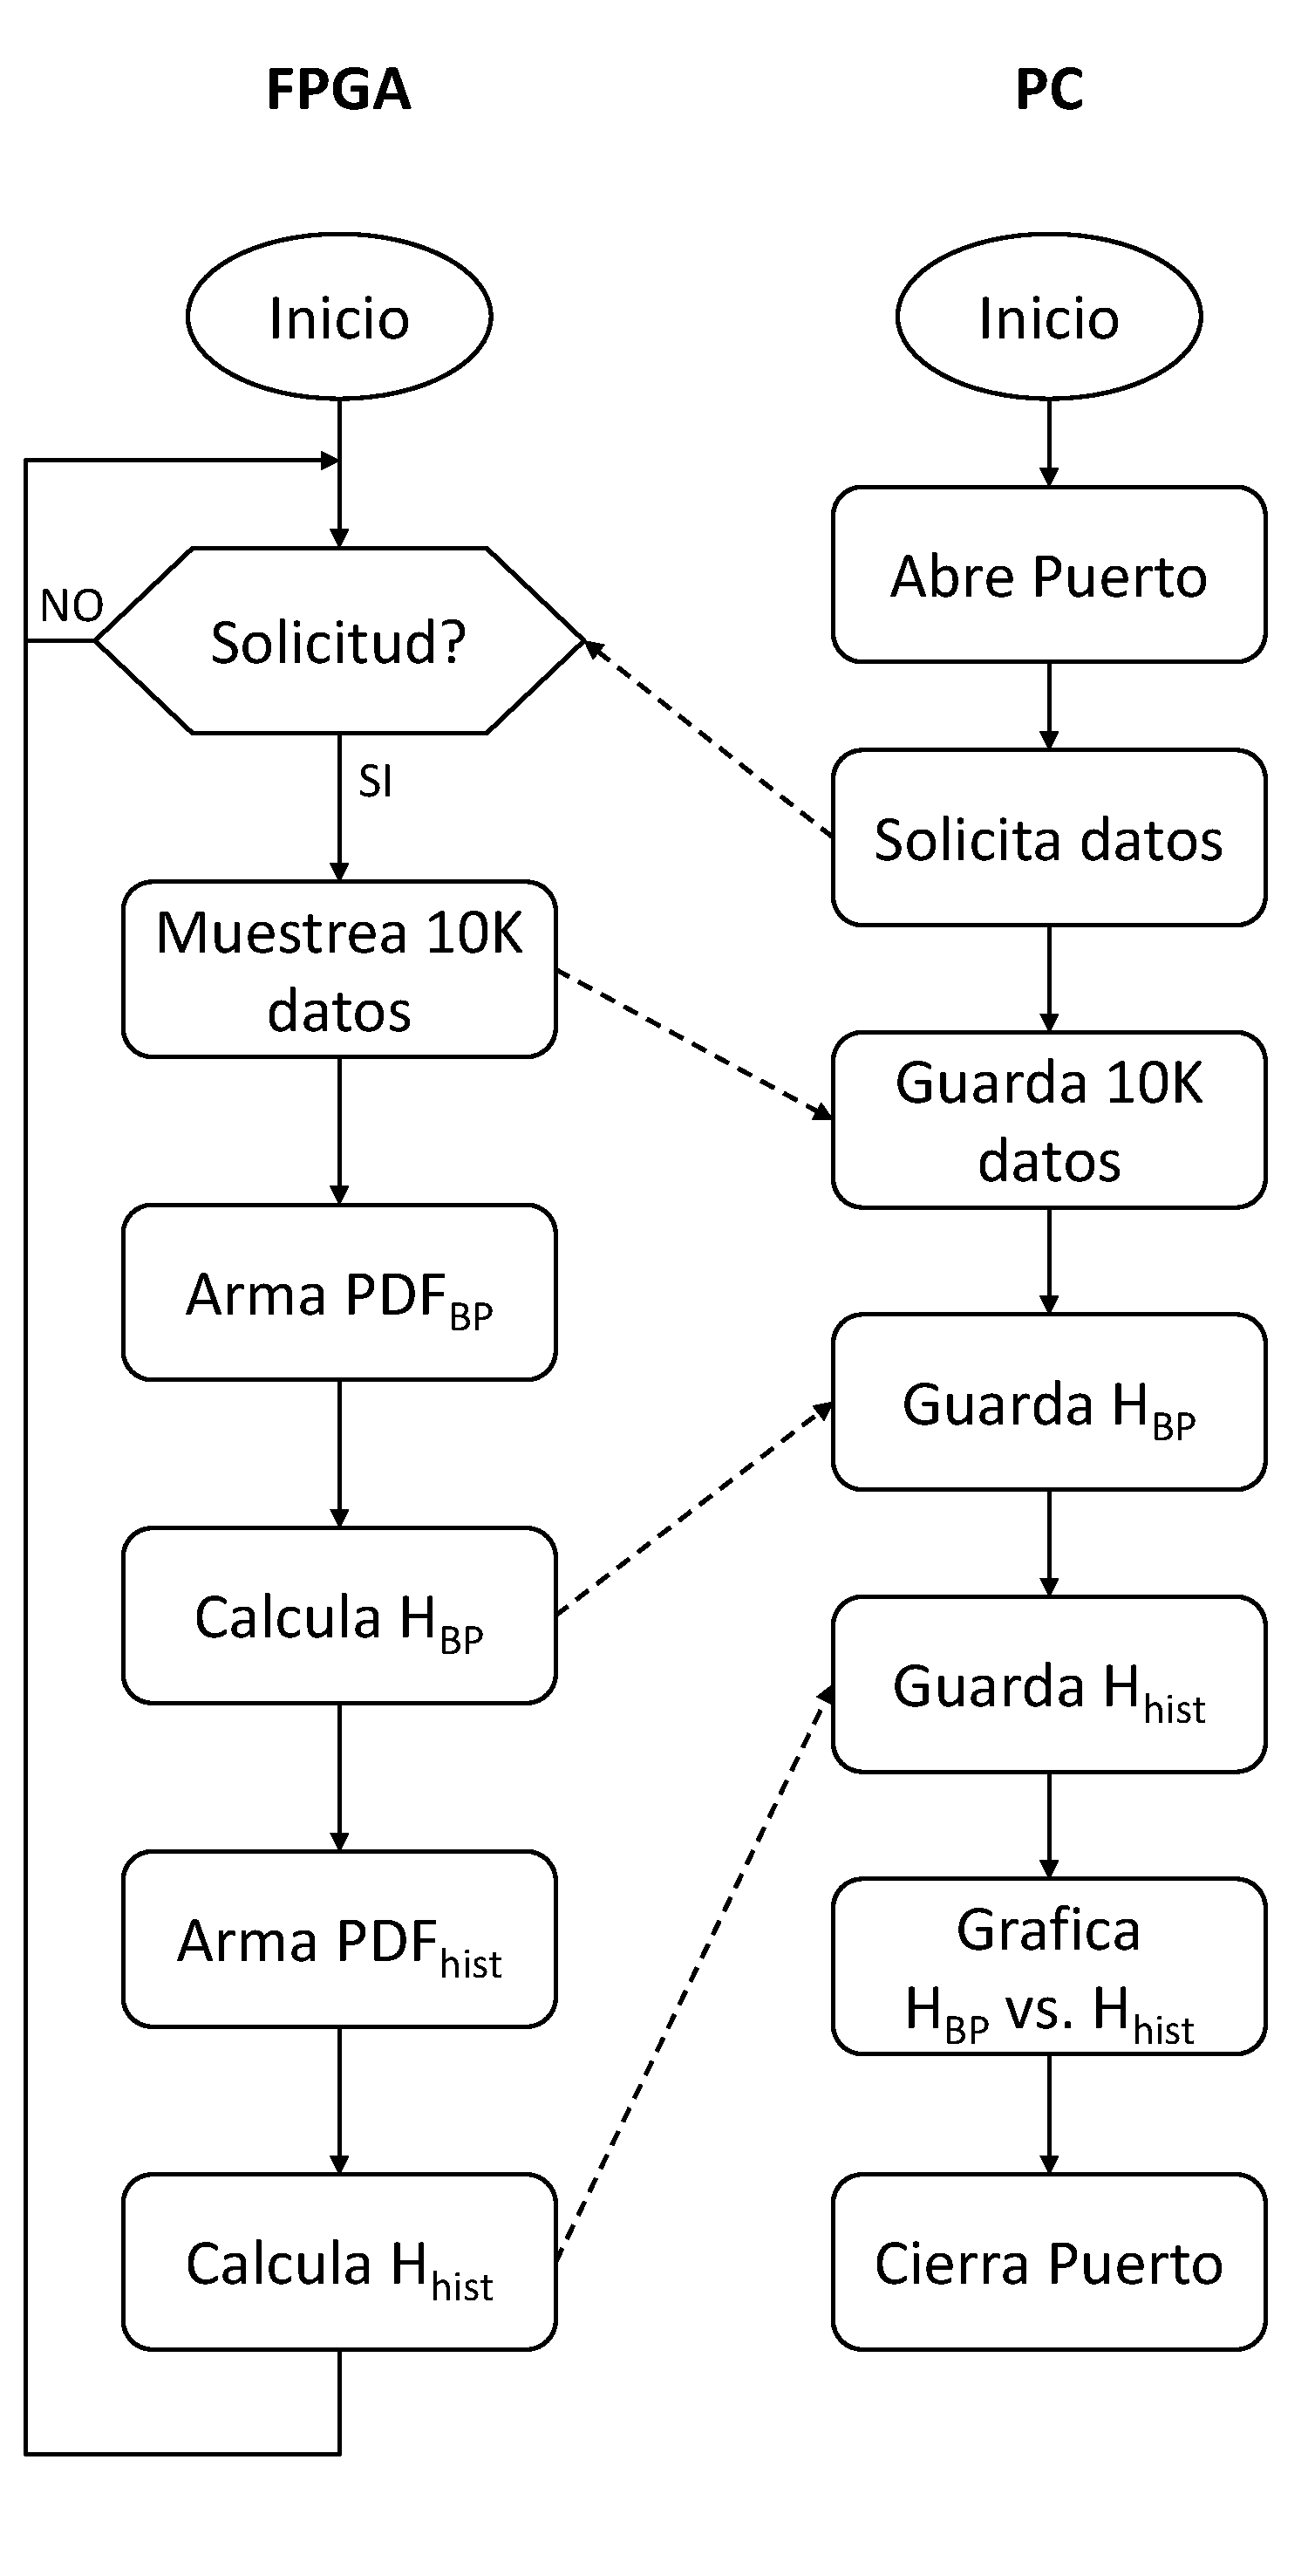
\includegraphics[width=0.7\columnwidth]{Soft}
	\caption{Diagrama de flujo del \textit{software} implementado.}\label{fig.softflow}
\end{figure}

En la PC corre un \textit{script} de Matlab que se encarga de abrir el puerto serie en donde se encuentra mapeado el USB, solicitar los datos, tomar los resultados del mismo puerto, graficarlos en un plano $H_{BP}$ vs. $H_{hist}$ y cerrar el puerto.

Sobre el microcontrolador en la FPGA corre un programa escrito en lenguaje C y compilado para el microcontrolador 8051 utilizando la herramienta \textit{SoftConsole~IDE~v3.4\textsuperscript\copyright}.
El firmware es una modificación del usado en \cite{Core8051sS}. Cuando se presenta una solicitud de datos por el puerto UART, se guardan los datos muestreados de la entrada analógica.
Luego, se recorre este vector generando las $PDF_{hist}$ y $PDF_{BP}$, a las que se les calcula sus respectivas entropías $H_{hist}$ y $H_{BP}$.
Estos resultados son enviados a la PC mediante el mismo puerto.

Con el fin de validar el sistema, el programa en la FPGA envía a  Matlab el vector de datos muestreados, para que se puedan calcular en la PC sus entropías y compararlas con los resultados del sistema implementado.

\subsubsection{Resultados}
\label{sec:resultados}

Como se dijo, para testear el sistema se compararon los resultados obtenidos por el sistema implementado y por un programa patrón que corre en la PC.
Para esto, se generaron $10~000$ muestras de señales con distintas formas de onda tanto externas (analógicas) como internas (digitales).

Las señales digitales fueron generadas por código en el microcontrolador, una corresponde a la función rand() de C y la otra al mapa caótico Logístico con parámetro r=4.

Las señales analógicas fueron generadas con el generador de funciones \textit{HP33120A}.
Tienen una amplitud de $4~Vpp$ y un nivel de continua de $2~V$ de forma de aprovechar todo el rango del conversor analógico-digital y aumentar la relación señal-ruido.
En los cuatro casos la frecuencia de las señales fue de $100~Hz$ y la velocidad de muestreo de $16~ks/s$.

El cuadro \ref{tablaErrores} muestra el error absoluto entre los resultados de los cuantificadores calculados en la FPGA comparados con los resultados calculados con el programa patrón sobre los mismos datos.
%
\begin{table}
	\centering
	\begin{tabular}{@{\extracolsep{\fill}}| c| c | c |c |}
		\hline
		\textbf{{Generador}} & \textbf{{Origen}} & \textbf{{Error}} \textbf{{$H_{BP}$}} & \textbf{\textbf{{Error}}} \textbf{{$H_{hist}$}} \\ \hline
		{Rand}               & {Digital}         & {$1,7421E^{-6}$}                     & {$2,6977E^{-6}$}                                \\ \hline
		{Logístico}          & {Digital}         & {$0,4256E^{-6}$}                     & {$94,693E^{-6}$}                                \\ \hline
		{Triangular}         & {Analógico}       & {$6,3445E^{-6}$}                     & {$2,0028EE^{-6}$}                               \\ \hline
		{Senoidal}           & {Analógico}       & {$6,3151E^{-6}$}                     & {$5,6506E^{-6}$}                                \\ \hline
		{Cuadrada}           & {Analógico}       & {$0,1797E^{-6}$}                     & {$1,9930EE^{-6}$}                               \\ \hline
		{Rampa}              & {Analógico}       & {$245,00E^{-6}$}                     & {$1,0876E^{-6}$}                                \\ \hline
	\end{tabular}
	\caption{Error de los cuantificadores evaluados en la FPGA con respecto a los resultados calculados por el programa patrón.}\label{tablaErrores}
\end{table}

La Figura \ref{fig:resultados} muestra los valores entregados por la FPGA en el plano $H_{BP}$ vs. $H_{hist}$.
%
\begin{figure}[htb]
	\centering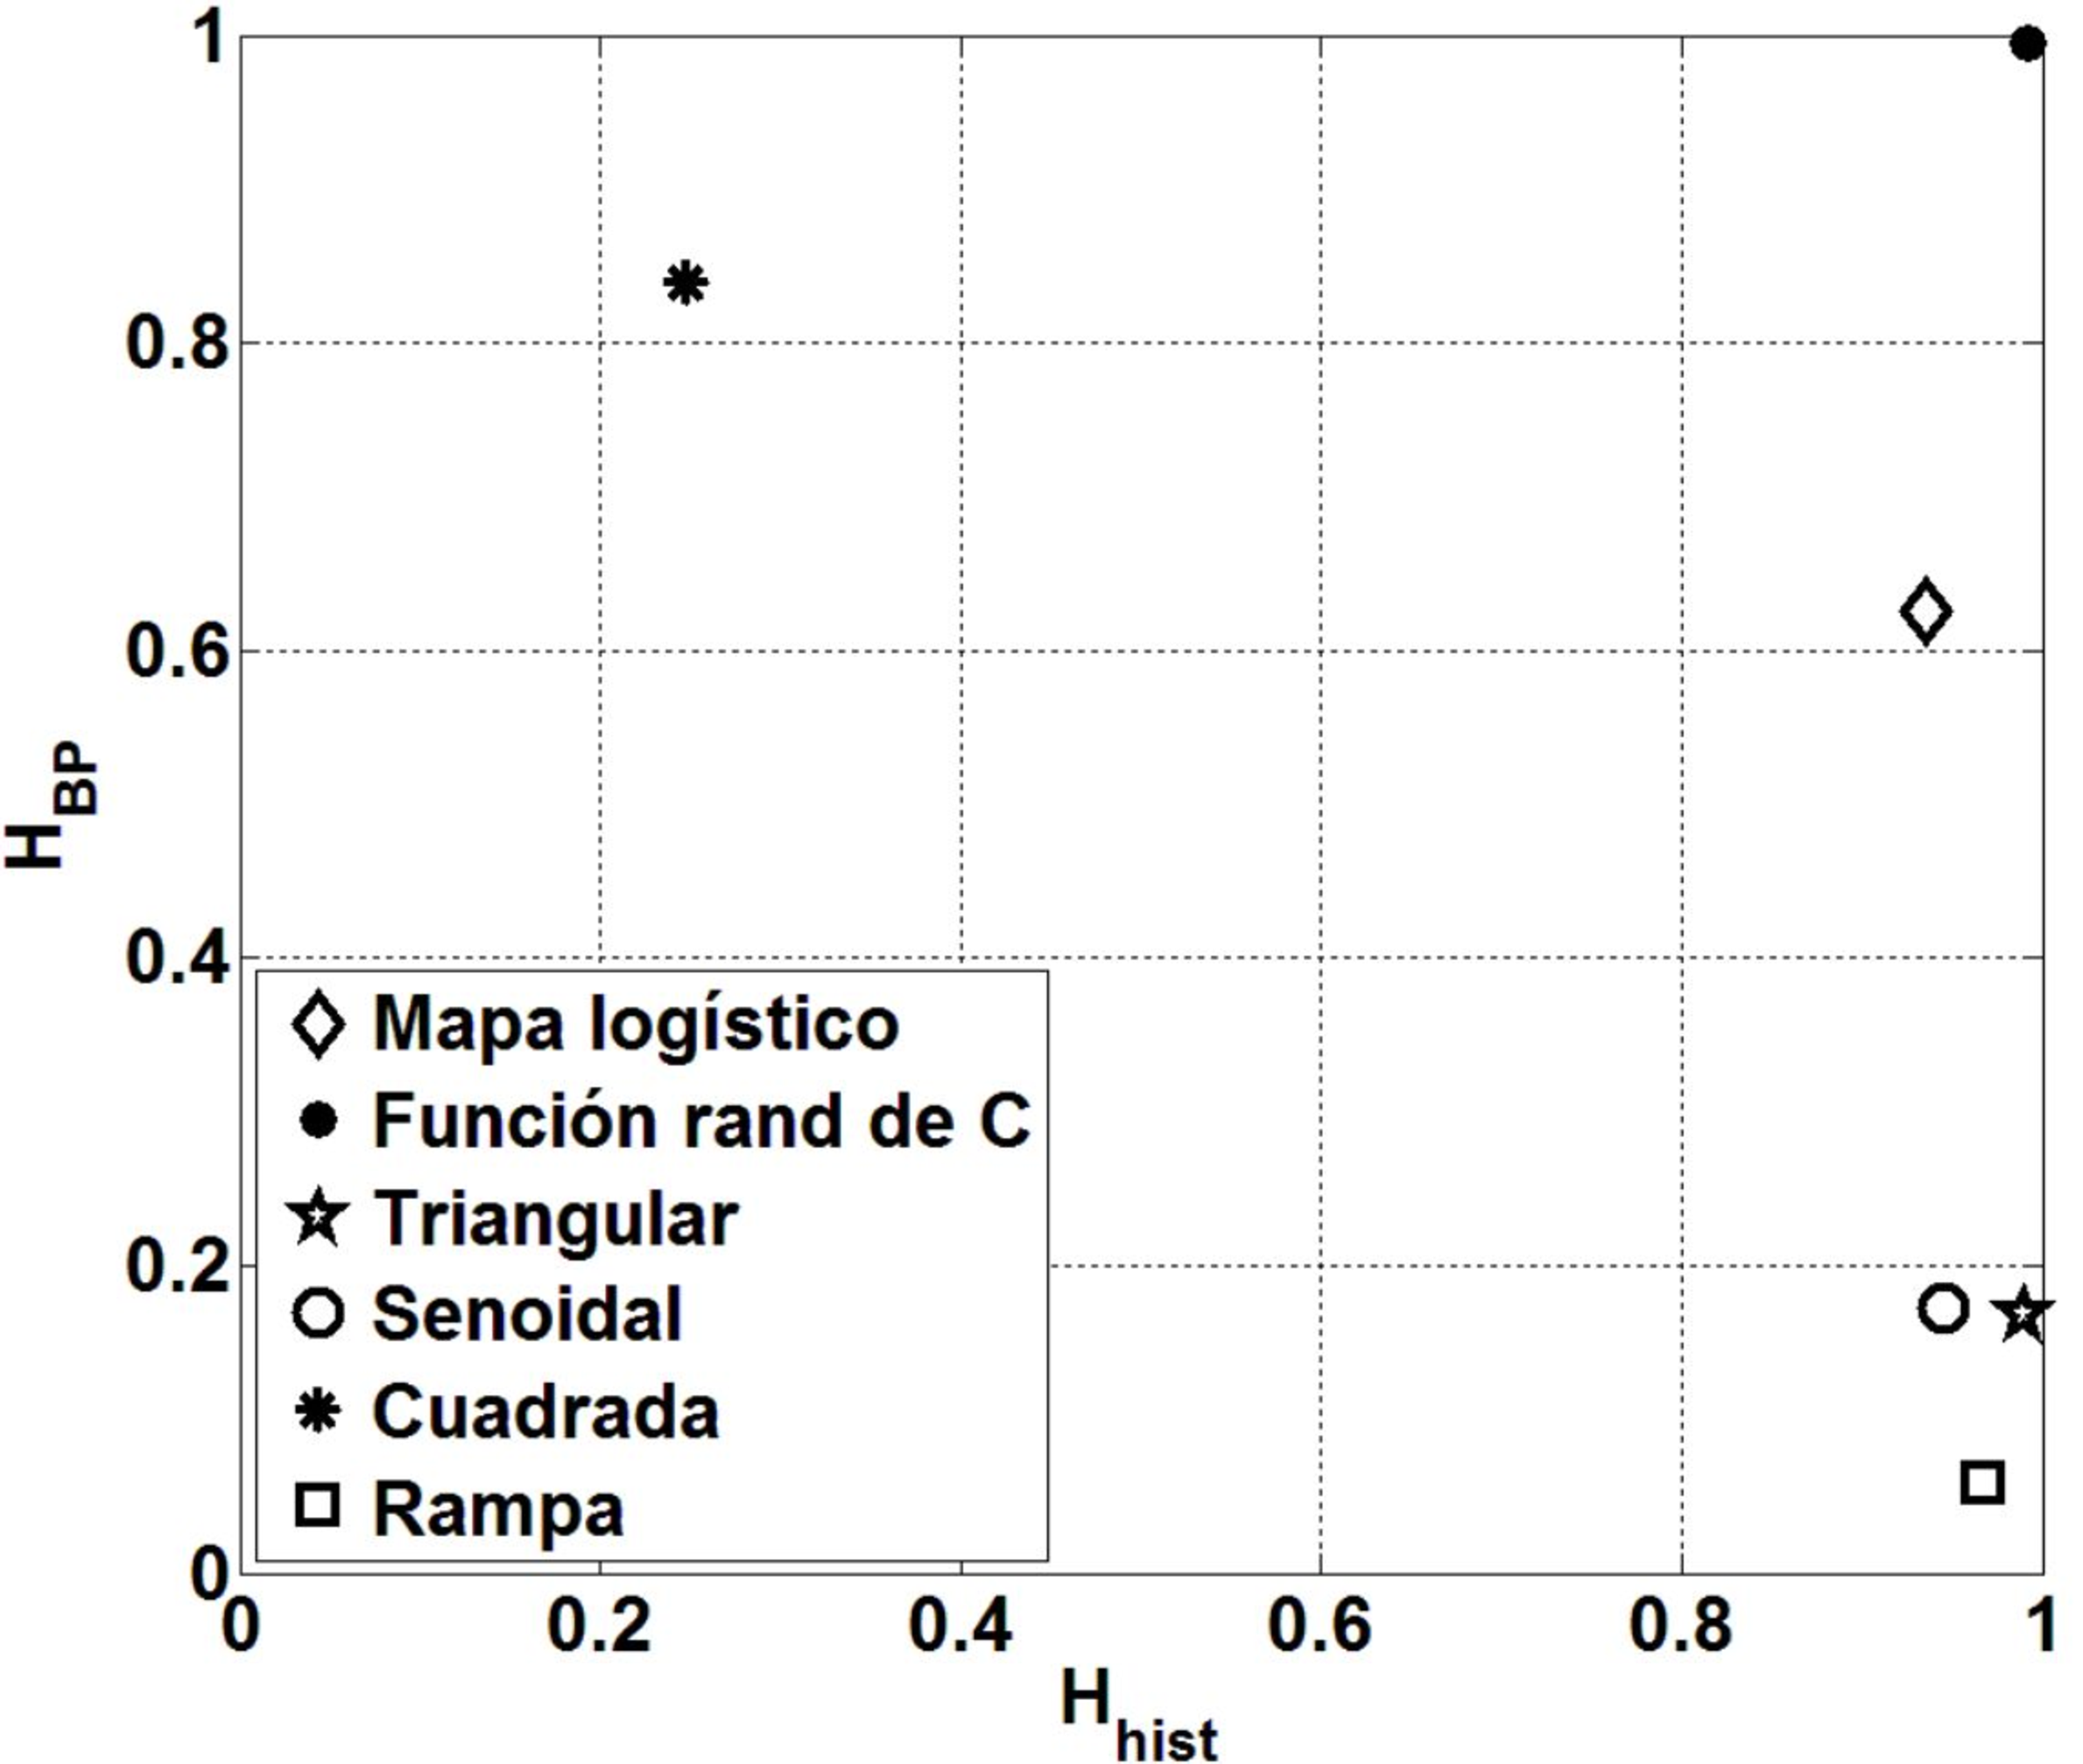
\includegraphics[width=.75\textwidth]{resultados}
	\caption{Resultados de las mediciones.}\label{fig:resultados}
\end{figure}

Los resultados de la compilación nos permiten conocer los recursos de la FPGA utilizados por el sistema completo y la cantidad de memoria ocupada por el \textit{software} que corre en el microcontrolador.
Recordemos que esta es una implementación de \textit{hardware} rígida, es decir primero se arma el circuito en la FPGA (microcontrolador, periféricos, etc.) y luego se carga el \textit{software} sobre él.

El reporte de la compilación de \textit{hardware} devuelto por el \textit{Place and Route} se muestra en la Figura \ref{fig:hard}. Podemos ver que la implementación utiliza un 19\% de los recursos lógicos de la FPGA, el $21\%$ de las celdas de entrada-salida y el $28\%$ de los bloques de memoria.
%
\begin{figure}[htb]
	\centering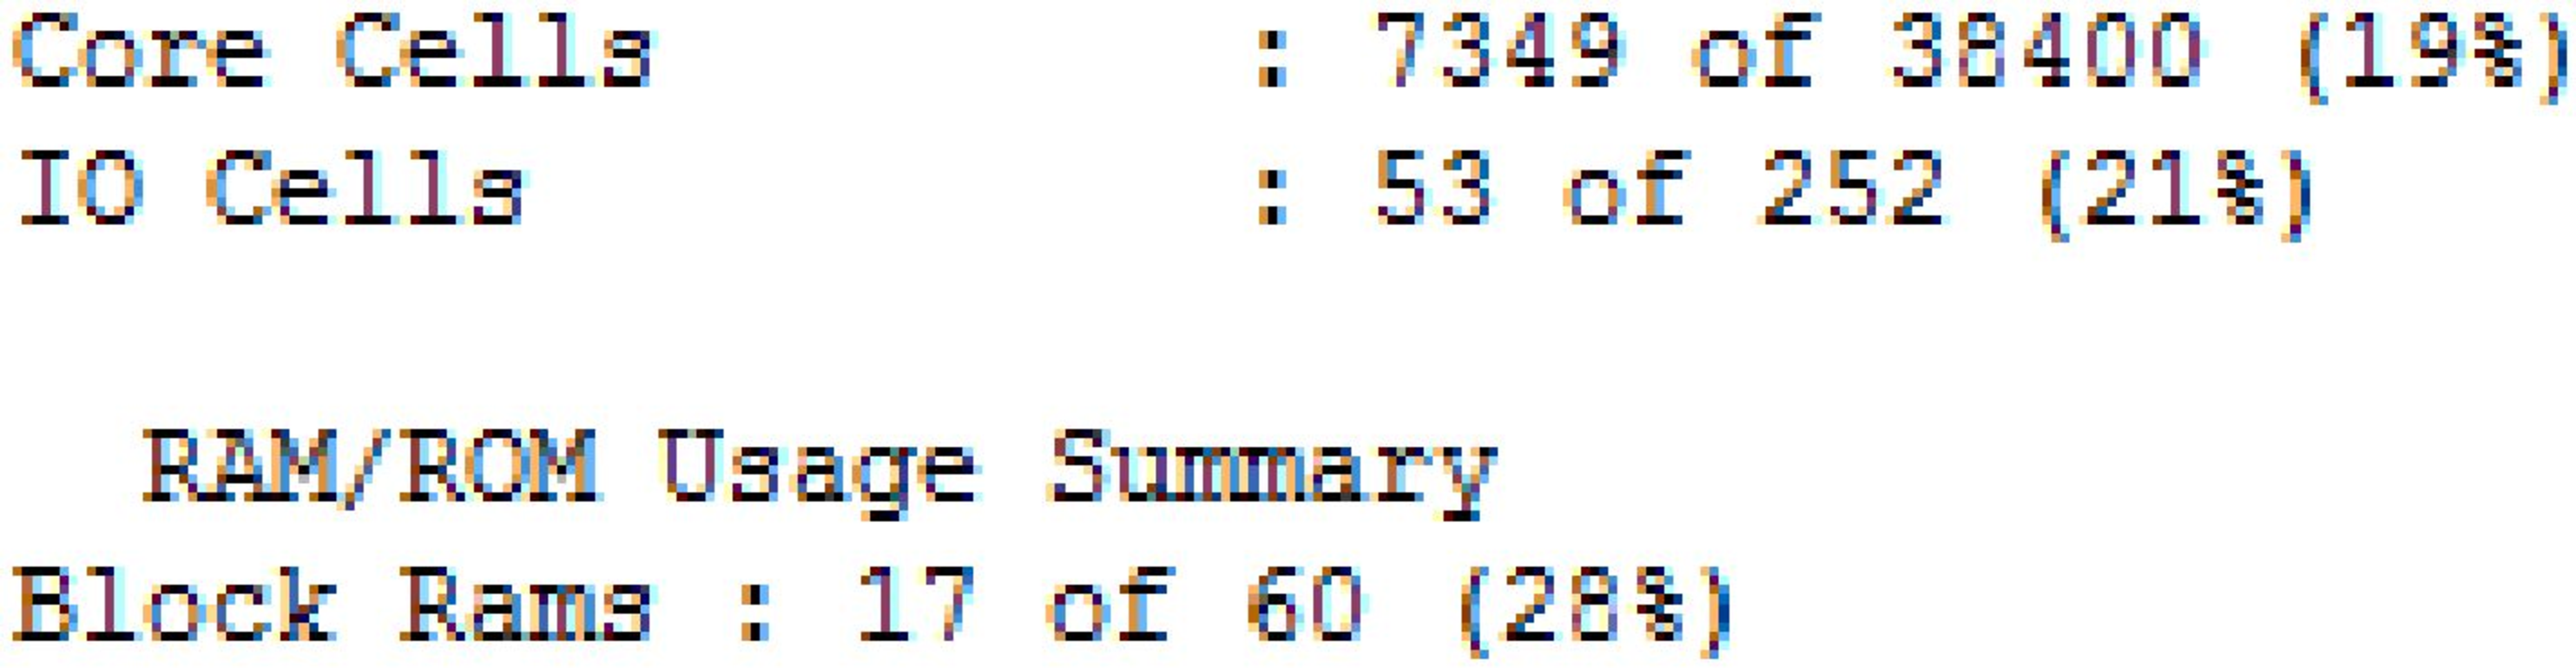
\includegraphics[scale=.13]{reporteHard}
	\caption{Recursos empleados por el \textit{hardware} del sistema.}\label{fig:hard}
\end{figure}

El reporte de la compilación de \textit{software} se muestra en la Figura \ref{fig:soft}.
Podemos ver que la memoria FLASH no volátil se encuentra ocupada al $15,4\%$.
Por otro lado, de las $47~145$ direcciones de memoria SRAM ocupada, $4~096$ son ocupadas por el bus APB y $43~049$ por las variables del programa.
%
\begin{figure}[htb]
	\centering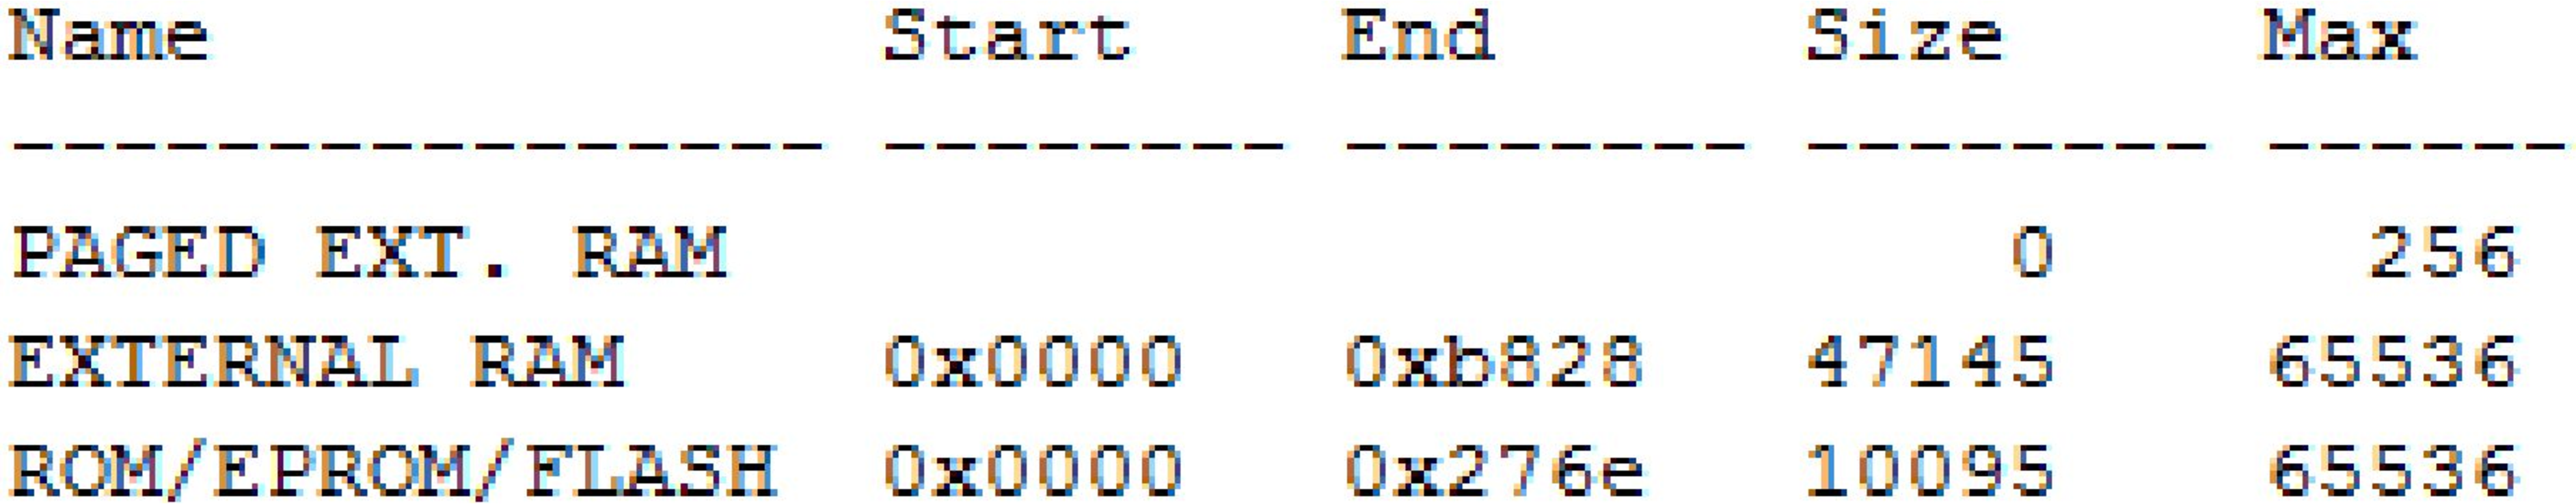
\includegraphics[scale=.13]{reporteSoft}
	\caption{Recursos empleados por el \textit{software} del sistema.}\label{fig:soft}
\end{figure}

El programa debió ser adaptado al microcontrolador instanciado en la FPGA.
Estas modificaciones hacen que la salida del sistema implementado no sea igual a la de un programa que corre en la PC, al cual tomamos como programa patrón.
Por esto se testeó el error cometido, para tener una cota y determinar si los resultados de los cuantificadores son correctos.
El programa patrón utiliza aritmética de $64~bits$ en punto flotante norma IEEE754-64~bits y emplea la librería math.h \cite{Mathe}.
Para el algoritmo en la FPGA se disminuyó la aritmética a 32 bits de punto flotante norma IEEE754-32~bits.
También se requirió el cálculo de la función logaritmo, que se implementó mediante un algoritmo de CORDIC.
En el Cuadro \ref{tablaErrores} se ve que el error absoluto no supera el sexto decimal, esto indica que se detecta diferencia recién a partir del quinto dígito decimal.

En la Figura \ref{fig:resultados} puede verse como los cuantificadores $H_{BP}$y $H_{hist}$ diferencian claramente las propiedades estadísticas de las series de datos analizadas.
Las señales Senoidal, Rampa y Triangular presentan un valor alto de $H_{hist}$ porque tienen casi todos los valores que es capaz de generar el conversor Analógico-Digital.
Sin embargo, la mezcla de estos datos es mala por tratarse de señales periódicas totalmente predecibles, esto se ve en el bajo valor de $H_{BP}$.
Un caso interesante de analizar es la señal Cuadrada.
El efecto del ruido aditivo es especialmente notable en las zonas en donde el valor de la señal debería ser constante.
Se generan dos Gaussianas muy finas en torno a los valores ideales en la $PDF_{hist}$, esto no afecta demasiado el valor calculado $H_{hist}$, sin embargo, para la $PDF_{BP}$, se calcula el patrón de orden directamente a la señal ruidosa, por lo que el valor de $H_{BP}$ es más alto que el esperado.
La señal generada mediante la función rand de C, presenta las mejores propiedades estadísticas ubicándose en el punto $\sim(1,1)$.